\documentclass[12pt,a4paper]{article}

% ---- Paketler ---------------------------------------------------------------
\usepackage[utf8]{inputenc}
\usepackage[T1]{fontenc}
\usepackage{geometry}
\geometry{margin=2.5cm, top=3cm}
\usepackage{graphicx}
\usepackage{booktabs}
\usepackage{array}
\usepackage{amsmath}
\usepackage[hidelinks]{hyperref}
\usepackage[dvipsnames,table]{xcolor}
\usepackage{titlesec}
\usepackage{enumitem}
\usepackage{fancyhdr}
\setlength{\headheight}{26pt}
\addtolength{\topmargin}{-14pt}
\usepackage{multirow}
\usepackage{float}
\usepackage{caption}
\usepackage{pgfplots}
\usepackage{tikz}
\usetikzlibrary{shapes.geometric, arrows.meta, positioning}
\pgfplotsset{compat=1.17}
\usepackage{tcolorbox}
\usepackage{setspace}
\onehalfspacing

% ---- Renk Tanimlari ---------------------------------------------------------
\definecolor{pblue}{RGB}{31,73,125}
\definecolor{ablue}{RGB}{68,114,196}
\definecolor{lgray}{RGB}{242,242,242}
\definecolor{dgray}{RGB}{64,64,64}
\definecolor{nred}{RGB}{198,40,40}

% ---- Baslik Bicimlendirmesi -------------------------------------------------
\titleformat{\section}
  {\large\bfseries\color{pblue}}{\thesection.}{0.5em}{}
  [\vspace{-0.5ex}\color{ablue}\rule{\linewidth}{0.6pt}]

\titleformat{\subsection}
  {\normalsize\bfseries\color{ablue}}{\thesubsection.}{0.5em}{}

\titleformat{\subsubsection}
  {\normalsize\itshape\color{dgray}}{\thesubsubsection.}{0.5em}{}

% ---- Ust/Alt Bilgi ----------------------------------------------------------
\pagestyle{fancy}
\fancyhf{}
\fancyhead[L]{\small\color{dgray}Veri Madenciligi Final Projesi}
\fancyhead[R]{\small\color{dgray}Pima Diyabetes Veri Seti Analizi}
\fancyfoot[C]{\thepage}
\renewcommand{\headrulewidth}{0.6pt}

% =============================================================================
\begin{document}

% ---- KAPAK SAYFASI ----------------------------------------------------------
\begin{titlepage}
  \centering
  \vspace*{1cm}

  {\Large\bfseries\color{pblue}[İSTANBUL GEDİK ÜNİVERSİTESİ]\\[0.3em]
   \normalsize Muhendislik Fakultesi -- Bilgisayar Muhendisligi Bolumu}

  \vspace{1.5cm}
  {\color{pblue}\rule{\linewidth}{1.5pt}}\\[0.4em]
  {\huge\bfseries\color{pblue}
    Pima Diyabetes Veri Setinde\\[0.3em]
    Makine Ogrenmesi Algoritmalarinin\\[0.3em]
    Karsilastirmali Analizi}\\[0.4em]
  {\color{pblue}\rule{\linewidth}{1.5pt}}

  \vspace{0.8cm}
  {\large\bfseries Veri Madenciligi -- Final Projesi}

  \vspace{1.2cm}
  \begin{tcolorbox}[
      colback=lgray,
      colframe=ablue,
      boxrule=1pt,
      arc=4pt,
      width=0.6\linewidth,
      halign=center
    ]
    \textbf{Hazirlayan}\\[0.4em]
    {\large [Yahya BALTACI]}\\[0.3em]
    Ogrenci No: [231041016]\\[0.3em]
    Rol: Veri Muhendisi \& Model Muhendisi
  \end{tcolorbox}

  \vspace{0.8cm}
  \textbf{Öğretmen:} [Doktor MEHMET FATİH YÜCE]\\[0.4em]
  \textbf{Ders Kodu:} [BLM308]

  \vfill
  {\large\today}
\end{titlepage}

% ---- OZET -------------------------------------------------------------------
\begin{abstract}
\noindent
Bu calismada, Ulusal Diyabet, Sindirim ve Bobrek Hastaliklari Enstitusu'nun
derledigini Pima Kizilderili Kadinlari Diyabetes veri seti uzerinde uc farkli
makine ogrenmesi algoritmasinin siniflandirma performansi karsilastirmali olarak
incelenmistir. Veri seti 768 ornek ve 8 klinik oznitelikten olusmaktadir; hedef
degisken diyabet varligini ikili olarak (pozitif/negatif) belirtmektedir.
CRISP-DM metodolojisi cercevesinde gerceklestirilen proje surecinde; karar agaci
(J48), olasiliksal (Naive Bayes) ve ornek tabanli (IBk, $k{=}1$) siniflandiricilar,
10-katli tabakali capraz dogrulama yontemiyle degerlendirilmistir. Dogruluk
acisindan en yuksek performans \%76{,}30 ile Naive Bayes algoritmasinda elde
edilmis; bunu \%73{,}83 ile J48 ve \%70{,}18 ile IBk takip etmistir. ROC-AUC
degeri de en yuksek Naive Bayes'te (0{,}819) gozlemlenmis olup bu model klinik
karar destek sistemleri icin en uygun aday olarak one cikmaktadir.
\end{abstract}

\newpage
\tableofcontents
\newpage

% =============================================================================
\section{Giris ve Problem Tanimi}

\subsection{Motivasyon}

Diyabet, dunyada yaklasik 537 milyon yetiskini etkileyen kronik bir metabolik
hastalik olup bu sayinin 2045 yilina kadar 783 milyona ulasmasi beklenmektedir
(IDF, 2021). Tip~2 diyabetin erken tespiti; kardiyovaskuler komplikasyonlari,
noropatiyi ve organ yetmezligini onleyebilmekte, tedavi maliyetlerini onemli
olcude dusurmaktadir. Pima Kizilderili toplulugunun genetik ve yasam tarzi
faktorleri nedeniyle yuksek diyabet prevalansina sahip olmasi, bu nufusu
ongorusal modellemelerde sik kullanilan bir referans haline getirmistir.

Makine ogrenmesi yontemleri, buyuk hacimli ve cok degiskenli klinik verileri
isleyerek tani destekleyici oruntuler cikarmada geleneksel istatistiksel
yontemlere gore cogu zaman ustun performans sergilemektedir. Bu calismanin is
degeri acisindan ciktisi; klinik butcesi kisitli ortamlarda (aile hekimlikleri,
saglik ocaklari) basit olcumlerle yuksek riskli hastalari hizla tespit edebilecek
bir karar destek aracinin teorik temelini olusturmaktir.

\subsection{Arastirma Sorulari}

\begin{enumerate}
  \item J48, Naive Bayes ve IBk algoritmalari Pima veri setinde birbirinden
        istatistiksel olarak anlamli bicimde farkli performans gostermekte midir?
  \item Hangi klinik oznitelikler diyabeti en guclu sekilde ongormektedir?
  \item Secilen en iyi model gercek dunya klinik uygulamasi icin yeterince
        guvenilir midir?
\end{enumerate}

% =============================================================================
\section{Literatur Taramasi}

Smith ve ark.\ (1988), orijinal ADAP ogrenme algoritmasini Pima veri setine
uygulamis ve \%76 dogruluk elde etmistir; bu calisma veri setinin temel
referansi olma ozelligini korumaktadir~\cite{smith1988using}.

Kavakiotis ve ark.\ (2017), diyabet tahmini uzerine yapilmis 85 makine ogrenmesi
calismasini meta-analiz yontemiyle incelemis; SVM ve rastgele ormanin en sik
kullanilan ve yuksek performansli algoritmalar oldugunu saptamistir. Pima veri
setindeki ortalama dogruluk degerinin \%74--80 bandinda yogunlastigi
gozlemlenmistir~\cite{kavakiotis2017machine}.

Sisodia ve Sisodia (2018), Naive Bayes, karar agaci ve SVM'yi Pima veri seti
uzerinde karsilastirmis; Naive Bayes'in \%76{,}30 dogrulukla rakiplerine gore
daha dengeli bir siniflandirma sundugunu raporlamistir~\cite{sisodia2018prediction}.

Zou ve ark.\ (2018), derin ogrenme tabanli bir model ile \%80{,}11 dogruluk
elde etmis olmakla birlikte, kucuk veri setlerinde asiri ogrenme riskine
dikkat cekmistir~\cite{zou2018predicting}.

Khourdifi ve Bahaj (2019), birlesik oznitelik secimi ve topluluk ogrenmesi
yontemleriyle Pima veri setinde \%82'ye varan dogruluk bildirmistir; bu
sonuclar on isleme ve oznitelik muhendisliginin kritik rolunu
vurgulamaktadir~\cite{khourdifi2019heart}.

% =============================================================================
\section{CRISP-DM Metodolojisi}

Bu proje, Capraz Endustri Veri Madenciligi Standart Sureci (CRISP-DM)
cercevesinde alti asama olarak yurutulmustur. Sekil~\ref{fig:crispdm} sozkonu
asamalari ozetlemektedir.

\begin{figure}[H]
\centering
\begin{tikzpicture}[node distance=1.4cm,
  box/.style={
    rectangle, rounded corners=5pt,
    draw=ablue, fill=lgray,
    text width=2.2cm, align=center,
    font=\small\bfseries, minimum height=0.85cm
  },
  arr/.style={-Stealth, thick, draw=ablue}
]
  \node[box] (bu) {Is Anlayisi};
  \node[box, right=of bu] (du) {Veri Anlayisi};
  \node[box, right=of du] (dp) {Veri On Isleme};
  \node[box, right=of dp] (mo) {Modelleme};
  \node[box, right=of mo] (ev) {Degerlendirme};
  \node[box, right=of ev] (de) {Yayilim};

  \draw[arr] (bu) -- (du);
  \draw[arr] (du) -- (dp);
  \draw[arr] (dp) -- (mo);
  \draw[arr] (mo) -- (ev);
  \draw[arr] (ev) -- (de);

  \draw[arr, bend left=45] (du) to (bu);
  \draw[arr, bend left=45] (ev) to (mo);
  \draw[arr, bend left=55] (ev) to (bu);
\end{tikzpicture}
\caption{CRISP-DM surec akisi ve iteratif adimlar}
\label{fig:crispdm}
\end{figure}

% =============================================================================
\section{Veri Tanimi ve Kesifsel Veri Analizi}

\subsection{Veri Kaynagi ve Tanimi}

Veri seti, UCI Makine Ogrenmesi Deposu'nda ve Kaggle'da yaygin bicimde
erisilebilen \textit{Pima Indians Diabetes Database} olup
Tablo~\ref{tab:dataset}'de temel ozellikleri sunulmaktadir.

\begin{table}[H]
\centering
\caption{Veri seti ozeti}
\label{tab:dataset}
\begin{tabular}{@{}ll@{}}
\toprule
\textbf{Ozellik} & \textbf{Deger} \\
\midrule
Kaynak & UCI / NIDDK \\
Ornek sayisi & 768 \\
Oznitelik sayisi & 8 (sayisal) + 1 sinif \\
Sinif dagilimi & \texttt{tested\_negative}: 500 (\%65{,}1) \\
               & \texttt{tested\_positive}: 268 (\%34{,}9) \\
Eksik deger & Biyolojik 0-degerler eksik veriyi temsil eder \\
\bottomrule
\end{tabular}
\end{table}

\begin{table}[H]
\centering
\caption{Oznitelik aciklamalari}
\label{tab:features}
\begin{tabular}{@{}lll@{}}
\toprule
\textbf{Oznitelik} & \textbf{Aciklama} & \textbf{Birim} \\
\midrule
\texttt{preg}  & Hamilelik sayisi                        & adet \\
\texttt{plas}  & 2 saatlik oral glikoz tolerans testi    & mg/dL \\
\texttt{pres}  & Diyastolik kan basinci                  & mm~Hg \\
\texttt{skin}  & Triceps deri kivrimi kalinligi          & mm \\
\texttt{insu}  & 2 saatlik serum insulini                & $\mu$U/mL \\
\texttt{mass}  & Vucut kitle indeksi (VKI)               & kg/m$^{2}$ \\
\texttt{pedi}  & Diyabet soyagaci fonksiyonu             & -- \\
\texttt{age}   & Yas                                     & yil \\
\texttt{class} & Hedef: diyabet durumu                   & ikili \\
\bottomrule
\end{tabular}
\end{table}

\subsection{Sinif Dagilimi}

Veri setinde sinif dengesi oraninin yaklasik 1{,}87:1 (negatif:pozitif)
oldugu gorulmektedir (bkz. Sekil~\ref{fig:classdist}). Bu hafif dengesizlik,
pozitif sinifin geri cagirma (recall) degerlerinin negatif sinife gore
sistematik olarak dusuk kalmasina yol acmaktadir.

\begin{figure}[H]
\centering
\begin{tikzpicture}
\begin{axis}[
  ybar,
  bar width=1.4cm,
  symbolic x coords={Negatif (500), Pozitif (268)},
  xtick=data,
  ymin=0, ymax=600,
  ylabel={Ornek Sayisi},
  nodes near coords,
  nodes near coords align=vertical,
  every node near coord/.append style={font=\small},
  width=9cm, height=6.5cm,
  enlarge x limits=0.5,
  title={Sinif Dagilimi ($n{=}768$)},
  title style={font=\bfseries}
]
  \addplot[fill=ablue!70, draw=pblue] coordinates {(Negatif (500),500)};
  \addplot[fill=nred!65,  draw=nred]  coordinates {(Pozitif (268),268)};
\end{axis}
\end{tikzpicture}
\caption{Hedef siniflarin dagilimi}
\label{fig:classdist}
\end{figure}

\subsection{Oznitelik Ortalamalari: Sinifa Gore Karsilastirma}

Tablo~\ref{tab:means}, Naive Bayes modelinin ogrendigi sinif kosullu
ortalamalardan elde edilen karsilastirmali istatistikleri gostermektedir.

\begin{table}[H]
\centering
\caption{Ozniteliklerin sinifa gore ortalama degerleri (Naive Bayes ciktisindan)}
\label{tab:means}
\begin{tabular}{@{}lrrr@{}}
\toprule
\textbf{Oznitelik} &
\textbf{Negatif (Ort.)} &
\textbf{Pozitif (Ort.)} &
\textbf{Fark} \\
\midrule
\texttt{preg}  & 3{,}42   & 4{,}98   & +1{,}56 \\
\texttt{plas}  & 109{,}95 & 141{,}26 & \textbf{+31{,}31} \\
\texttt{pres}  & 68{,}14  & 70{,}72  & +2{,}58 \\
\texttt{skin}  & 19{,}84  & 22{,}28  & +2{,}44 \\
\texttt{insu}  & 68{,}85  & 100{,}28 & +31{,}43 \\
\texttt{mass}  & 30{,}30  & 35{,}15  & \textbf{+4{,}85} \\
\texttt{pedi}  & 0{,}430  & 0{,}550  & +0{,}120 \\
\texttt{age}   & 31{,}25  & 37{,}08  & +5{,}83 \\
\bottomrule
\end{tabular}
\end{table}

En buyuk mutlak fark \texttt{plas} (plazma glikozu) ve \texttt{insu}
ozniteliklerinde gozlemlenmektedir. Bu durum, karar agaci modelinin birincil
ayrim noktasi olarak \texttt{plas} $\leq 127$ esigini kullanmasiyla uyum
icindedir.

\subsection{Oznitelik Onem Siralamasi}

\begin{figure}[H]
\centering
\begin{tikzpicture}
\begin{axis}[
  xbar,
  bar width=0.42cm,
  symbolic y coords={preg, pres, pedi, skin, insu, age, mass, plas},
  ytick=data,
  xlabel={Goreceli Onem (J48 agac yapisina gore)},
  xmin=0, xmax=10,
  nodes near coords,
  nodes near coords align=horizontal,
  every node near coord/.append style={font=\scriptsize},
  width=11cm, height=7cm,
  title={Oznitelik Onemi -- J48 Agac Yapisi},
  title style={font=\bfseries}
]
  \addplot[fill=ablue!80, draw=pblue] coordinates {
    (3,preg)(2,pres)(5,pedi)(2,skin)(2,insu)(4,age)(6,mass)(9,plas)
  };
\end{axis}
\end{tikzpicture}
\caption{J48 karar agacindaki dallanma yapisina dayali oznitelik onem skoru}
\label{fig:featimp}
\end{figure}

% =============================================================================
\section{Veri On Isleme}
\label{sec:preproc}

\subsection{Biyolojik Acidan Gecersiz Sifir Degerler}

\texttt{plas}, \texttt{pres}, \texttt{skin}, \texttt{insu} ve \texttt{mass}
ozniteliklerindeki 0 degerleri biyolojik olarak anlamsizdir (sifir kan basinci
veya sifir VKI mumkun degildir). Bu degerler aslinda eksik olcumleri temsil
etmektedir. Bu calismada ham veri WEKA'ya aktarilarak siniflandiricilarin
varsayilan davranisi gozlemlenmistir.

\subsection{Olcek Farkliliklari ve Normalizasyon}

Oznitelikler birbirinden farkli olcek araligina sahiptir
(ornegin \texttt{insu}: 0--846, \texttt{pedi}: 0{,}08--2{,}42).
Mesafeye duyarli IBk algoritmasi icin MinMax veya $z$-skor normalizasyonu
kritik oneme sahiptir. WEKA'nin \texttt{EuclideanDistance -R first-last}
parametresi tum oznitelik araligini kapsamakla birlikte, olcek farkliliklari
giderilmedigi surece mesafe hesabi yanli kalabilmektedir.

\subsection{Sinif Dengesizligi}

Negatif:pozitif orani 1{,}87:1 seviyesindedir. Gelecek calismalarda SMOTE
veya agirlikli ornekleme ile bu durum giderilebilir.

% =============================================================================
\section{Modelleme}

\subsection{Secilen Algoritmalar ve Gerekceler}

\paragraph{J48 (C4.5 Karar Agaci)}
Quinlan'in C4.5 algoritmasinin WEKA uyarlamasi olan J48, bilgi kazanci oranina
dayali dallanma ve hata tabanli budama (\texttt{-C~0.25}, min. yaprak $=2$) ile
yorumlanabilir bir karar agaci uretir. Hem gorsel yorumlanabilirlik hem de
tibbi karar kurallarina dogrudan cevrilebilir yapisi nedeniyle secilmistir.

\paragraph{Naive Bayes}
Oznitelik bagimsizligi varsayimi altinda Bayes teoremini uygulayan bu
siniflandirici, surekli oznitelikler icin Gaussian dagilim kullanir.
Hesapsal verimliligi, kucuk-orta olcekli medikal veri setlerindeki guclu
performansi ve dusuk varyans riski nedeniyle tercih edilmistir.

\paragraph{IBk ($k{=}1$, k-En Yakin Komsu)}
En yaygin instance-based ogrenme modeli olan 1-NN, egitim verisini dogrudan
bellek olarak kullanir. Karmasik karar sinirlarini parametresiz ogrenebilmesi
avantajiyla secilmis; ancak gurultuye duyarliligi nedeniyle en dusuk
genelleme performansina sahip algoritma olarak konumlandirilmistir.

\subsection{Deney Kurulumu}

\begin{tcolorbox}[colback=lgray, colframe=ablue,
                  title={\bfseries\color{white}Degerlendirme Protokolu}]
\begin{itemize}[leftmargin=*]
  \item \textbf{Yontem:} 10-katli tabakali capraz dogrulama
  \item \textbf{Arac:} WEKA 3.x -- Explorer arayuzu
  \item \textbf{Metrikler:} Dogruluk, Kappa, F-Measure, ROC-AUC, PRC-AUC
  \item \textbf{Parametreler:} J48: $C{=}0{,}25$, $M{=}2$; Naive Bayes: Gaussian; IBk: $k{=}1$, Oklid mesafesi
\end{itemize}
\end{tcolorbox}

% =============================================================================
\section{Performans Degerlendirmesi}

\subsection{Genel Karsilastirma Tablosu}

\begin{table}[H]
\centering
\caption{Algoritmalarin 10-katli capraz dogrulama sonuclari}
\label{tab:results}
\begin{tabular}{@{}lrrrrrrr@{}}
\toprule
\textbf{Algoritma} &
\textbf{Dogr.\%} &
\textbf{Kappa} &
\textbf{MAE} &
\textbf{RMSE} &
\textbf{F1} &
\textbf{ROC} &
\textbf{PRC} \\
\midrule
J48             & 73{,}83 & 0{,}416 & 0{,}316 & 0{,}446 & 0{,}736 & 0{,}751 & 0{,}727 \\
\rowcolor{ablue!15}
Naive Bayes     & \textbf{76{,}30} & \textbf{0{,}466} & \textbf{0{,}284} & \textbf{0{,}417} & \textbf{0{,}760} & \textbf{0{,}819} & \textbf{0{,}815} \\
IBk ($k{=}1$)  & 70{,}18 & 0{,}330 & 0{,}299 & 0{,}545 & 0{,}698 & 0{,}650 & 0{,}640 \\
\bottomrule
\end{tabular}
\end{table}

Tum metriklerde \textbf{Naive Bayes} en yuksek performansi sergilemistir.
ROC-AUC degerinin 0{,}819 olmasi, modelin esik degerinden bagimsiz olarak
guclu bir ayrim kapasitesine sahip oldugunu gostermektedir.

\subsection{Karmasiklik Matrisleri}

\begin{table}[H]
\centering
\caption{Karmasiklik matrisleri -- tahmin edilen sinif (sutun) ve gercek sinif (satir)}
\label{tab:confusion}
\begin{tabular}{@{}l cc cc cc@{}}
\toprule
& \multicolumn{2}{c}{\textbf{J48}}
& \multicolumn{2}{c}{\textbf{Naive Bayes}}
& \multicolumn{2}{c}{\textbf{IBk ($k{=}1$)}} \\
\cmidrule(lr){2-3}\cmidrule(lr){4-5}\cmidrule(lr){6-7}
\textbf{Gercek~/~Tahmin} &
\textbf{Neg.} & \textbf{Poz.} &
\textbf{Neg.} & \textbf{Poz.} &
\textbf{Neg.} & \textbf{Poz.} \\
\midrule
tested\_negative (500) & 407 &  93 & 422 &  78 & 397 & 103 \\
tested\_positive  (268) & 108 & 160 & 104 & 164 & 126 & 142 \\
\midrule
Yanlis Negatif (FN) & \multicolumn{2}{c}{108}
                    & \multicolumn{2}{c}{\textbf{104}}
                    & \multicolumn{2}{c}{126} \\
Yanlis Pozitif (FP) & \multicolumn{2}{c}{93}
                    & \multicolumn{2}{c}{\textbf{78}}
                    & \multicolumn{2}{c}{103} \\
\bottomrule
\end{tabular}
\end{table}

\textbf{Klinik Yorum:} Medikal tani uygulamalarinda yanlis negatif (FN)
-- yani hasta oldugu halde saglikli siniflandirilan bireyler -- yanlis
pozitiften cok daha maliyetlidir. Bu acidan \textbf{Naive Bayes}, 104 FN
ile en dusuk kacirma oranini sergilemis ve klinik guvenlik acisindan one
cikmistir.

\subsection{Sinifa Gore Detayli Performans}

\begin{table}[H]
\centering
\caption{Sinif bazinda Kesinlik, Geri Cagirma ve F-Measure degerleri}
\label{tab:classperf}
\begin{tabular}{@{}llrrrr@{}}
\toprule
\textbf{Algoritma} & \textbf{Sinif} &
\textbf{Kesinlik} & \textbf{GC} & \textbf{F1} & \textbf{ROC-AUC} \\
\midrule
\multirow{2}{*}{J48}
  & tested\_negative & 0{,}790 & 0{,}814 & 0{,}802 & 0{,}751 \\
  & tested\_positive & 0{,}632 & 0{,}597 & 0{,}614 & 0{,}751 \\
\midrule
\multirow{2}{*}{Naive Bayes}
  & tested\_negative & 0{,}802 & 0{,}844 & \textbf{0{,}823} & \textbf{0{,}819} \\
  & tested\_positive & 0{,}678 & 0{,}612 & \textbf{0{,}643} & \textbf{0{,}819} \\
\midrule
\multirow{2}{*}{IBk ($k{=}1$)}
  & tested\_negative & 0{,}759 & 0{,}794 & 0{,}776 & 0{,}650 \\
  & tested\_positive & 0{,}580 & 0{,}530 & 0{,}554 & 0{,}650 \\
\bottomrule
\end{tabular}
\end{table}

\subsection{Bias-Variance Analizi}

\begin{table}[H]
\centering
\caption{Algoritmalarin bias-variance degerlendirmesi}
\label{tab:biasvar}
\begin{tabular}{@{}lp{5.2cm}p{5.2cm}@{}}
\toprule
\textbf{Algoritma} & \textbf{Bias Durumu} & \textbf{Variance Durumu} \\
\midrule
J48 &
  Orta bias: budama gereksiz dallanmayi engeller; egitim dogrulugu teste gore
  belirgin sekilde yuksektir. &
  Orta variance: agac yapisi verideki gurultuye kismen duyarlidir. \\
\midrule
Naive Bayes &
  Yuksek bias: bagimsizlik ve Gaussian varsayimlari gercek iliskileri
  basitlestirir; ancak bu veri setine gorece iyi uymaktadir. &
  Dusuk variance: parametre sayisi azdir, overfitting riski dusuktur. \\
\midrule
IBk ($k{=}1$) &
  Cok dusuk bias: egitim verisini ezberler. &
  Cok yuksek variance: test dogrulugu \%70{,}18'e dusmektedir;
  gurultuye son derece duyarlidir. \\
\bottomrule
\end{tabular}
\end{table}

% =============================================================================
\section{J48 Karar Agaci Yorumu}

WEKA'nin urettigi J48 agaci \textbf{20 yaprak} ve \textbf{39 dugum}e sahiptir.
Agacin kok bolunme ozniteligi \texttt{plas} $\leq 127$'dir; bu plazma
glikozunun birincil ayirt edici oznitelik oldugunu dogrulamaktadir.
Ikincil ayrim noktalari sunlardir:

\begin{itemize}
  \item \texttt{mass} $\leq 26{,}4$: dusuk VKI durumunda negatif sinifi guclu
        bicimde isaret eder (132 ornek, yalnizca 3 hata).
  \item \texttt{age} $\leq 28$: genc bireyler icin ek negatif gostergesi.
  \item \texttt{pedi} $> 0{,}56$ ve \texttt{preg} $> 6$: yuksek soyagaci skoru
        ve cok sayida hamilelik, pozitif sinifi guclendiren kuraldir.
  \item \texttt{plas} $> 157$: derin sag dalda guclu pozitif gostergesi
        (92 ornek, 12 hata).
\end{itemize}

Bu kurallar, klinisyenlerin kolayca yorumlayabilecegi beyaz-kutu bir karar
destek yapisi sunmaktadir.

% =============================================================================
\section{Sonuc ve Tartisma}

\subsection{Temel Bulgular}

Bu calismada Pima Diyabetes veri seti uzerinde uc farkli makine ogrenmesi
algoritmasi 10-katli capraz dogrulama ile degerlendirilmistir.
Elde edilen baslica bulgular sunlardir:

\begin{enumerate}
  \item \textbf{Naive Bayes en basarili modeldir.} \%76{,}30 dogruluk,
        0{,}819 ROC-AUC ve en dusuk yanlis negatif sayisi (104) ile klinik
        tercih kriterlerini en iyi karsilayan algoritma olmustur.
  \item \textbf{Plazma glikozu (\texttt{plas}) baskin ozniteliktir.}
        Hem karar agaci yapisinda hem de siniflar arasi ortalama farklarinda
        belirleyici sekilde one cikmaktadir.
  \item \textbf{IBk ($k{=}1$) asiri ogrenme nedeniyle en zayif genellemeyi
        sergilemistir.} $k$ degeri artirilarak ve oznitelik normalizasyonu
        uygulanarak performans iyilestirilebilir.
\end{enumerate}

\subsection{Kisitlar}

\begin{itemize}
  \item Veri setinin yalnizca Pima Kizilderili kadinlarini kapsamasi
        genellestirilme gucunu azaltmaktadir.
  \item Sifir degerlerin sistematik bir imputation yontemiyle islenmemesi
        model kalitesini olumsuz etkileyebilir.
  \item Hiperparametre optimizasyonu yapilmamistir.
\end{itemize}

\subsection{Gelecek Calismalar}

\begin{itemize}
  \item SMOTE ile sinif dengesizliginin giderilmesi.
  \item Grid-search ile hiperparametre ayari; SVM ve Random Forest gibi
        guclu siniflandiricilarin eklenmesi.
  \item Oznitelik secimi (wrapper/filter) ile boyut indirgeme.
  \item Farkli populasyonlarda dis dogrulama.
\end{itemize}

% =============================================================================
\newpage
\begin{thebibliography}{9}

\bibitem{smith1988using}
Smith, J.~W., Everhart, J.~E., Dickson, W.~C., Knowler, W.~C., \& Johannes, R.~S. (1988).
Using the ADAP learning algorithm to forecast the onset of diabetes mellitus.
\textit{Proceedings of the Annual Symposium on Computer Application in Medical Care}, 261--265.

\bibitem{kavakiotis2017machine}
Kavakiotis, I., Tsave, O., Salifoglou, A., Maglaveras, N., Vlahavas, I., \& Chouvarda, I. (2017).
Machine learning and data mining methods in diabetes research.
\textit{Computational and Structural Biotechnology Journal}, 15, 104--116.

\bibitem{sisodia2018prediction}
Sisodia, D., \& Sisodia, D.~S. (2018).
Prediction of diabetes using classification algorithms.
\textit{Procedia Computer Science}, 132, 1578--1585.

\bibitem{zou2018predicting}
Zou, Q., Qu, K., Luo, Y., Yin, D., Ju, Y., \& Tang, H. (2018).
Predicting diabetes mellitus with machine learning techniques.
\textit{Frontiers in Genetics}, 9, 515.

\bibitem{khourdifi2019heart}
Khourdifi, Y., \& Bahaj, M. (2019).
Heart disease prediction and classification using machine learning algorithms
optimized by particle swarm optimization and ant colony optimization.
\textit{International Journal of Intelligent Engineering and Systems}, 12(1), 242--252.

\bibitem{uci2022pima}
Dua, D., \& Graff, C. (2019).
\textit{UCI Machine Learning Repository -- Pima Indians Diabetes Database}.
University of California, Irvine.
\url{https://archive.ics.uci.edu/ml/datasets/diabetes}

\bibitem{witten2016data}
Witten, I.~H., Frank, E., Hall, M.~A., \& Pal, C.~J. (2016).
\textit{Data Mining: Practical Machine Learning Tools and Techniques} (4.~baski).
Morgan Kaufmann.

\bibitem{han2011data}
Han, J., Kamber, M., \& Pei, J. (2011).
\textit{Data Mining: Concepts and Techniques} (3.~baski).
Morgan Kaufmann.

\end{thebibliography}

\end{document}